\documentclass[aspectratio=169, 11pt, t, xcolor={table}]{beamer}
% Slides of the English course "Computer Architecture" (same theme as the
% ENSB decks: light background, teal + orange). Compile from en/slides/.
\usepackage{amsmath, amssymb}
\usepackage{booktabs, colortbl, tabularx, array}
\usepackage{tikz}
\usepackage[skins]{tcolorbox}
\usepackage{fontawesome5}
\usepackage{listings}
\usepackage{fontspec}
\usetikzlibrary{positioning, calc, arrows.meta, shapes.geometric, decorations.pathreplacing}

\setsansfont{texgyreheros}[Extension=.otf, UprightFont=*-regular, BoldFont=*-bold,
    ItalicFont=*-italic, BoldItalicFont=*-bolditalic]
\newfontfamily\codefont[Scale=0.95, BoldFont=lmmonolt10-bold.otf,
    ItalicFont=lmmono10-italic.otf]{lmmono10-regular.otf}

\definecolor{brandTeal}{HTML}{5CC8E6}
\definecolor{brandOrange}{HTML}{FFA27F}
\definecolor{brandLight}{HTML}{F8F9FA}
\definecolor{brandDark}{HTML}{263238}
\definecolor{brandMuted}{HTML}{6C757D}
\definecolor{brandGreen}{HTML}{7BC47F}
\definecolor{brandPurple}{HTML}{B39DDB}
\colorlet{tealDeep}{brandTeal!60!black}
\colorlet{orangeDeep}{brandOrange!70!black}
\definecolor{codeGrey}{HTML}{F1F3F5}

\setbeamercolor{background canvas}{bg=brandLight}
\setbeamercolor{normal text}{fg=brandDark}
\setbeamercolor{structure}{fg=brandTeal}
\setbeamertemplate{navigation symbols}{}
\setbeamertemplate{frametitle}{%
    \vspace{0.35cm}
    \noindent{\bfseries\Large\color{brandDark}\insertframetitle}\par
    \vskip-2pt\noindent{\color{brandTeal}\rule{\textwidth}{1.5pt}}\vspace{0.05cm}}
\setbeamertemplate{footline}{%
    \hbox to \paperwidth{\hspace{0.6cm}{\color{brandMuted}\scriptsize\insertshorttitle}\hfill
        {\color{brandMuted}\scriptsize\insertframenumber\,/\,\inserttotalframenumber}\hspace{0.6cm}}%
    \vspace{0.25cm}}
\setbeamertemplate{itemize item}{\color{brandTeal}\small\faChevronRight}
\setbeamertemplate{itemize subitem}{\color{brandMuted}\small\faAngleRight}
\setbeamertemplate{enumerate item}{\color{tealDeep}\bfseries\insertenumlabel.}
% list lines are 1.4 cm apart (baseline to baseline)
\newlength{\lineGap}\setlength{\lineGap}{1.4cm}
\let\origlist\list
\def\list#1#2{\origlist{#1}{#2\setlength{\itemsep}{\dimexpr\lineGap-\baselineskip\relax}\setlength{\parsep}{0pt}}}

\newcolumntype{L}{>{\raggedright\arraybackslash}X}
\newcolumntype{C}{>{\centering\arraybackslash}X}
\newcommand{\ras}[1]{\cellcolor{brandTeal!20}\textbf{#1}}
\newcommand{\cell}[2]{\leavevmode\textcolor{#1}{#2}}
\renewcommand{\arraystretch}{1.3}
\setlength{\arrayrulewidth}{0.6pt}
\arrayrulecolor{brandMuted!70}

\tcbset{brandbox/.style={enhanced, arc=4pt, outer arc=4pt, boxrule=1.5pt,
    coltitle=white, coltext=brandDark, fonttitle=\bfseries,
    toptitle=0.8mm, bottomtitle=0.8mm, top=1.2mm, bottom=1.2mm, left=3mm, right=3mm,
    before skip=4pt, after skip=4pt}}
\newtcolorbox{tbox}[2][]{brandbox, colback=brandTeal!10, colframe=brandTeal, title={#2}, #1}
\newtcolorbox{obox}[2][]{brandbox, colback=brandOrange!10, colframe=brandOrange, title={#2}, #1}
\newtcolorbox{gbox}[2][]{brandbox, colback=brandGreen!8, colframe=brandGreen, title={#2}, #1}
\newtcolorbox{pbox}[2][]{brandbox, colback=brandPurple!10, colframe=brandPurple, title={#2}, #1}

\newcommand{\code}[1]{\mbox{\codefont\color{tealDeep}#1}}
\newcommand{\hex}[1]{\mbox{#1\textsubscript{H}}}
\newcommand{\bin}[1]{\mbox{#1\textsubscript{2}}}
\newcommand{\nql}[2]{\mbox{#1\,$\leftarrow$\,#2}}

% ---- code from ../../code/ (the verified programs of the course) ----
\lstdefinelanguage{asm86}{
    morekeywords={mov, add, adc, sub, sbb, inc, dec, neg, mul, imul, div, idiv,
        cmp, and, or, xor, not, test, shl, shr, sal, sar, rol, ror, jmp, je, jne,
        jz, jnz, jg, jge, jl, jle, ja, jae, jb, jbe, jcxz, loop, call, ret, iret,
        int, push, pop, lea, xchg, in, out, nop, movsb, rep, cld, std, cli, sti,
        syscall, addps, vaddps},
    morekeywords=[2]{org, db, dw, dd, dq, equ, proc, endp, offset, ptr, byte,
        word, dword, qword, section, global, dup, resb, rel},
    sensitive=false, morecomment=[l]{;}, morestring=[b]', morestring=[b]"}
\lstdefinestyle{base}{basicstyle=\codefont\fontsize{8}{8.6}\selectfont, columns=fullflexible,
    keepspaces=true, showstringspaces=false, upquote=true,
    keywordstyle=\color{tealDeep}\bfseries, keywordstyle=[2]\color{brandPurple!60!black}\bfseries,
    commentstyle=\color{red!75!black}, stringstyle=\color{orangeDeep},
    numbers=left, numberstyle=\tiny\color{brandMuted}, numbersep=7pt,
    firstnumber=auto,  % excerpts keep the real line numbers of the book
    xleftmargin=16pt, aboveskip=0pt, belowskip=0pt}
\lstdefinestyle{asm}{style=base, language=asm86}
\lstdefinestyle{c}{style=base, language=C}
\newtcolorbox{codebox}{enhanced, colback=codeGrey, colframe=codeGrey, boxrule=0pt, arc=2pt,
    left=3pt, right=3pt, top=2pt, bottom=2pt, before skip=3pt, after skip=3pt,
    overlay={\fill[brandTeal!70] (frame.south west) rectangle ([xshift=2.5pt]frame.north west);}}
\newtcolorbox{outbox}{enhanced, colback=brandDark, colframe=brandDark, boxrule=0pt, arc=2pt,
    left=5pt, right=5pt, top=2pt, bottom=2pt, before skip=3pt, after skip=3pt, colupper=white}
% \asm[firstline=5, lastline=20]{ch3/procnum.asm}   \cfile{...}   \screen{ch3/hello.out}
% assembly on slides: copies in code/ with inline comments removed (same lines,
% same numbers as the book; the explanation is on the slide)
\newcommand{\asm}[2][]{\begin{codebox}\lstinputlisting[style=asm,#1]{code/#2}\end{codebox}}
% smaller code for programs with long comments
\newcommand{\codesize}{\codefont\fontsize{7}{7.5}\selectfont}
\newcommand{\asms}[2][]{\begin{codebox}\lstinputlisting[style=asm,basicstyle=\codesize,#1]{code/#2}\end{codebox}}
\newcommand{\cfiles}[2][]{\begin{codebox}\lstinputlisting[style=c,basicstyle=\codesize,#1]{../../code/#2}\end{codebox}}
\newcommand{\cfile}[2][]{\begin{codebox}\lstinputlisting[style=c,#1]{../../code/#2}\end{codebox}}
\newcommand{\screen}[2][]{\begin{outbox}\lstinputlisting[basicstyle=\codefont\fontsize{8}{8.6}\selectfont\color{white},
    columns=fullflexible, keepspaces=true, aboveskip=0pt, belowskip=0pt,#1]{../../code/#2}\end{outbox}}

\tikzset{
    sahm/.style={-{Stealth[length=2.4mm]}, thick, color=brandMuted},
    sahmT/.style={-{Stealth[length=2.4mm]}, very thick, color=tealDeep},
    sahmO/.style={-{Stealth[length=2.4mm]}, very thick, color=orangeDeep},
    unit/.style={draw=#1, fill=#1!15, very thick, rounded corners=4pt,
        align=center, font=\bfseries\small, inner sep=4pt, text=brandDark},
    unit/.default=brandTeal,
    reg/.style={draw=brandDark, fill=white, thick, minimum height=0.6cm,
        font=\codefont\small, inner sep=2pt},
    % styles with a colour argument must be defined here, not inside a frame
    layer/.style={draw=#1, fill=#1!15, very thick, minimum width=9cm, minimum height=0.7cm, font=\small},
    evo/.style={unit=#1, minimum width=2.6cm, minimum height=1.2cm, font=\small},
}

% Title slide: \cover{Chapter 1}{Title}{subtitle}
\newcommand{\cover}[3]{%
\begin{frame}[plain]
    \begin{tikzpicture}[remember picture, overlay]
        \draw[brandTeal, line width=1.5pt, opacity=0.3] (current page.south east) ++(-1,1) circle (4cm);
        \draw[brandTeal, line width=0.8pt, opacity=0.25] (current page.north west) ++(2,2) circle (6cm);
        \draw[brandOrange, line width=0.5pt, opacity=0.25] (current page.north west) ++(2,2) circle (7cm);
        \begin{scope}[shift={([xshift=-1.6cm, yshift=-1.4cm]current page.north east)}, scale=0.35]
            \fill[brandDark] (-1.5,-1.5) rectangle (1.5,1.5);
            \fill[brandTeal] (-1,-1) rectangle (1,1);
            \foreach \i in {-1.2,-0.6,0,0.6,1.2} {
                \draw[brandMuted, line width=1pt] (\i,1.5) -- (\i,2); \draw[brandMuted, line width=1pt] (\i,-1.5) -- (\i,-2);
                \draw[brandMuted, line width=1pt] (1.5,\i) -- (2,\i); \draw[brandMuted, line width=1pt] (-1.5,\i) -- (-2,\i);}
        \end{scope}
    \end{tikzpicture}
    \vspace{1.4cm}
    \begin{minipage}{0.85\textwidth}
        {\color{tealDeep}\bfseries Computer Architecture \textbullet\ #1}\\[0.3cm]
        {\color{brandDark}\LARGE\bfseries #2\par}\vspace{0.3cm}
        {\color{brandMuted}\large #3}
    \end{minipage}
    \vspace{1.2cm}
    \begin{minipage}{0.85\textwidth}
        \color{brandMuted}\small
        \begin{tabular}{@{}ll}
            \textbf{Teacher:} & Dr. Benabderrezak Youcef \\
            \textbf{Course:} & UEF31, Architecture des ordinateurs \\
        \end{tabular}
    \end{minipage}
\end{frame}}

\title[Ch. 4: 32-bit and 64-bit processors]{Case Study: 32-bit and 64-bit Processors}

\begin{document}

\cover{Chapter 4}{Case Study: 32-bit and 64-bit Processors}{IA-32, AMD64, registers, flat addressing, SSE/AVX, pipeline}

\begin{frame}{Goals of this chapter}
    \begin{tbox}{\faBullseye\quad At the end, you can:}
        \begin{itemize}
            \item explain what changed from 16 to 32 and 64 bits;
            \item use the 64-bit registers and the base + index $\times$ scale addressing;
            \item explain SIMD instructions and the pipeline.
        \end{itemize}
    \end{tbox}
\end{frame}

\begin{frame}{16, 32 or 64 bits?}
    \begin{center}
    \small
    \begin{tabular}{|l|c|c|c|}
        \hline \ras{} & \ras{8086} & \ras{IA-32} & \ras{x86-64} \\ \hline
        register size & 16 & 32 & 64 \\ \hline
        max memory & 1 MB & 4 GB & 256 TB (48 bits) \\ \hline
        general registers & 8 & 8 & \textbf{16} \\ \hline
        names & AX & EAX & RAX, \dots, R15 \\ \hline
        addressing & segmented & flat & flat \\ \hline
    \end{tabular}
    \end{center}
    An \textbf{$n$-bit} processor has $n$-bit general registers.
\end{frame}

\begin{frame}{Why more than 32 bits?}
    \begin{enumerate}
        \item \textbf{Memory}: 32-bit addresses stop at 4 GB.
        \item \textbf{Performance}: big numbers in one instruction, and 16 registers.
        \item \textbf{Compatibility}: old 32-bit programs still run.
    \end{enumerate}
    \begin{gbox}{\faShoePrints\quad 4 GB exactly}
        $2^{32} = 2^2 \times 2^{30} = 4$ GB \qquad and \qquad $2^{48} = 2^8 \times 2^{40} = 256$ TB.
    \end{gbox}
\end{frame}

\begin{frame}{From IA-32 to AMD64}
    \begin{center}
    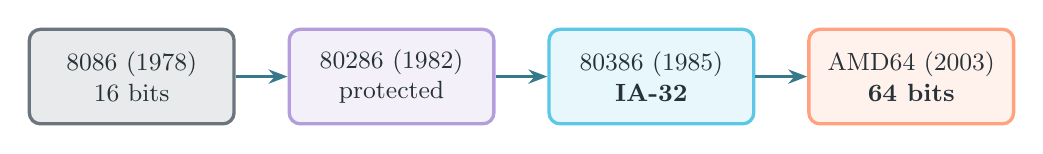
\begin{tikzpicture}
        \node[evo=brandMuted] (a) at (0,0) {8086 (1978)\\16 bits};
        \node[evo=brandPurple] (b) at (3.3,0) {80286 (1982)\\protected};
        \node[evo=brandTeal] (c) at (6.6,0) {80386 (1985)\\\textbf{IA-32}};
        \node[evo=brandOrange] (d) at (9.9,0) {AMD64 (2003)\\\textbf{64 bits}};
        \draw[sahmT] (a) -- (b); \draw[sahmT] (b) -- (c); \draw[sahmT] (c) -- (d);
    \end{tikzpicture}
    \end{center}
    \begin{center}
    \small
    \begin{tabular}{|l|l|}
        \hline \ras{Mode} & \ras{Description} \\ \hline
        real & like an 8086, at start-up \\ \hline
        protected & 32 bits, memory protection \\ \hline
        long & 64 bits, plus a 32-bit compatibility sub-mode \\ \hline
    \end{tabular}
    \end{center}
\end{frame}

\begin{frame}{Nested registers}
    \begin{center}
    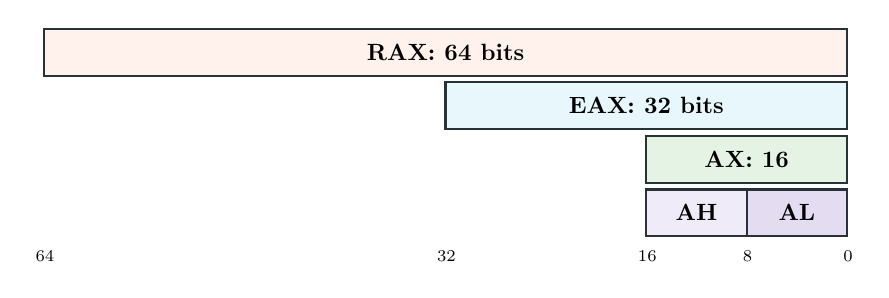
\begin{tikzpicture}[scale=0.85, transform shape, b/.style={draw=brandDark, thick, minimum height=0.7cm, font=\codefont\bfseries}]
        \node[b, minimum width=12cm, fill=brandOrange!15, anchor=east] at (6,1.6) {RAX: 64 bits};
        \node[b, minimum width=6cm, fill=brandTeal!15, anchor=east] at (6,0.8) {EAX: 32 bits};
        \node[b, minimum width=3cm, fill=brandGreen!20, anchor=east] at (6,0) {AX: 16};
        \node[b, minimum width=1.5cm, fill=brandPurple!20, anchor=east] at (4.5,-0.8) {AH};
        \node[b, minimum width=1.5cm, fill=brandPurple!35, anchor=east] at (6,-0.8) {AL};
        \foreach \x/\t in {6/0, 4.5/8, 3/16, 0/32, -6/64} \node[font=\codefont\scriptsize] at (\x,-1.45) {\t};
    \end{tikzpicture}
    \end{center}
    New: \textbf{R8 to R15}, \textbf{RIP}, \textbf{RFLAGS}.\\ Parameters: RDI, RSI, RDX, RCX; result: RAX.
\end{frame}

\begin{frame}{A test: what happens to the other bits?}
    \begin{columns}[T]
        \column{0.55\textwidth}
        \asm[firstline=4, firstnumber=4, lastline=18]{ch4/regs64.asm}
        \column{0.42\textwidth}
        \screen{ch4/regs64.out}
        \begin{obox}{\faExclamationTriangle\quad Rule}
            Writing a \textbf{32-bit} register clears the high 32 bits. Writing 8 or 16 bits keeps them.
        \end{obox}
    \end{columns}
\end{frame}

\begin{frame}{From segments to a flat memory}
    \begin{center}
    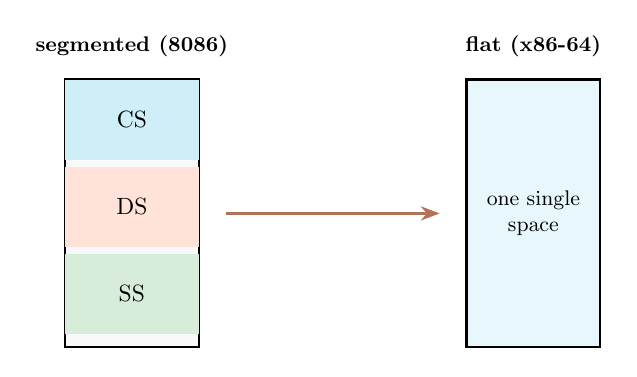
\begin{tikzpicture}[scale=0.85, transform shape]
        \draw[thick, fill=brandLight] (-6,0) rectangle (-4,-4);
        \foreach \y/\c in {0/brandTeal, -1.3/brandOrange, -2.6/brandGreen} \fill[\c!30] (-6,\y) rectangle (-4,\y-1.2);
        \foreach \y/\t in {-0.6/CS, -1.9/DS, -3.2/SS} \node[font=\codefont] at (-5,\y) {\t};
        \node[font=\small\bfseries] at (-5,0.5) {segmented (8086)};
        \draw[thick, fill=brandTeal!15] (0,0) rectangle (2,-4);
        \node[font=\small, align=center] at (1,-2) {one single\\space};
        \node[font=\small\bfseries] at (1,0.5) {flat (x86-64)};
        \draw[sahmO] (-3.6,-2) -- (-0.4,-2);
    \end{tikzpicture}
    \end{center}
    In the \textbf{flat model}, an address is just one number in a 64-bit register.
\end{frame}

\begin{frame}{The general form of an address}
    \begin{tbox}{\faLightbulb\quad Rule}
        \centering address $=$ base $+$ index $\times$ scale $+$ displacement \quad (scale: 1, 2, 4 or 8)
    \end{tbox}
    \begin{center}
    \small
    \begin{tabular}{|l|l|}
        \hline \ras{NASM} & \ras{Use} \\ \hline
        \code{[rbx]} & a pointer \\ \hline
        \code{[rbx + 16]} & a field in a struct \\ \hline
        \code{[tab + rcx*8]} & element i of an array of 8-byte numbers \\ \hline
        \code{[rel msg]} & relative to RIP (64 bits only) \\ \hline
    \end{tabular}
    \end{center}
    \code{[tab + rcx*8]} with RCX = 3 reads $3 \times 8 = 24$ bytes after \code{tab}.
\end{frame}

\begin{frame}{Example: the sum of an array}
    \begin{columns}[T]
        \column{0.55\textwidth}
        \asm[firstline=4, firstnumber=4, lastline=16]{ch4/sum64.asm}
        \column{0.42\textwidth}
        \small
        \begin{itemize}
            \item Line 8: scaled index.
            \item Lines 9--11: \code{while (i < 5)}.
        \end{itemize}
        \screen{ch4/sum64.out}
    \end{columns}
\end{frame}

\begin{frame}{RIP-relative addressing}
    \begin{itemize}
        \item \code{lea rsi, [rel buf]}: the address is $\text{RIP} + \text{distance}$.
        \item The program works \textbf{wherever} the system loads it.
        \item This helps security: the system moves programs at each run.
    \end{itemize}
\end{frame}

\begin{frame}{The same instruction on 16, 32 and 64 bits}
    \begin{center}
    \begin{tabular}{|l|l|l|}
        \hline \ras{Instruction} & \ras{Machine code (real)} & \ras{Note} \\ \hline
        \code{add ax, bx} & {\codefont \textcolor{orangeDeep}{66} 01 D8} & prefix 66: 16 bits \\ \hline
        \code{add eax, ebx} & {\codefont 01 D8} & default size \\ \hline
        \code{add rax, rbx} & {\codefont \textcolor{orangeDeep}{48} 01 D8} & REX.W: 64 bits \\ \hline
        \code{add r8, r9} & {\codefont \textcolor{orangeDeep}{4D} 01 C8} & REX: new registers \\ \hline
    \end{tabular}
    \end{center}
    01 D8 is the same since the 8086: the new sizes come from a \textbf{prefix}.
\end{frame}

\begin{frame}{32 bits or 64 bits: hello}
    \begin{columns}[T]
        \column{0.49\textwidth}
        \asms[firstline=8, firstnumber=8, lastline=17]{ch4/hello32.asm}
        \screen{ch4/hello32.out}
        \column{0.49\textwidth}
        \asms[firstline=8, firstnumber=8, lastline=17]{ch4/hello64.asm}
        \screen{ch4/hello64.out}
    \end{columns}
    \small 32 bits: \code{int 0x80}, write = 4, parameters EBX, ECX, EDX. \quad 64 bits: \code{syscall}, write = 1, parameters RDI, RSI, RDX.
\end{frame}

\begin{frame}{What does the compiler write?}
    \begin{columns}[T]
        \column{0.48\textwidth}
        \cfile{ch4/sum.c}
        \small \code{gcc -O1 -S -masm=intel sum.c}
        \column{0.48\textwidth}
        \asms{ch4/sum_gcc.s}
    \end{columns}
    \small \code{t} arrives in RDI, \code{n} in RSI; the result goes back in RAX.
\end{frame}

\begin{frame}{SIMD: one instruction, several numbers}
    \begin{center}
    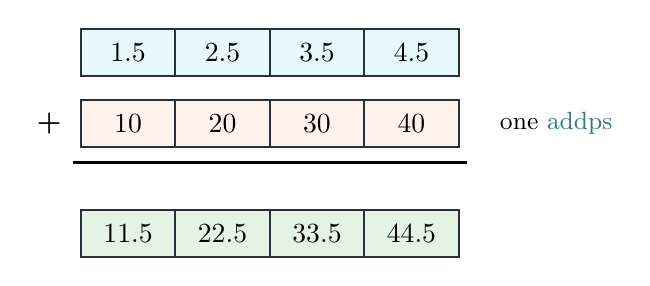
\begin{tikzpicture}[c/.style={draw=brandDark, thick, minimum width=1.2cm, minimum height=0.6cm, font=\codefont}]
        \foreach \v [count=\i from 0] in {1.5, 2.5, 3.5, 4.5} \node[c, fill=brandTeal!15] at (1.2*\i,1.5) {\v};
        \foreach \v [count=\i from 0] in {10, 20, 30, 40} \node[c, fill=brandOrange!15] at (1.2*\i,0.6) {\v};
        \foreach \v [count=\i from 0] in {11.5, 22.5, 33.5, 44.5} \node[c, fill=brandGreen!20] at (1.2*\i,-0.8) {\v};
        \draw[very thick] (-0.7,0.1) -- (4.3,0.1);
        \node[font=\bfseries] at (-1,0.6) {+};
        \node[font=\small, anchor=west] at (4.6,0.6) {one \code{addps}};
    \end{tikzpicture}
    \end{center}
    \begin{center}
    \small
    \begin{tabular}{|c|c|c|c|}
        \hline \ras{Extension} & \ras{Registers} & \ras{Size} & \ras{floats at once} \\ \hline
        SSE & XMM & 128 bits & 4 \\ \hline
        AVX & YMM & 256 bits & 8 \\ \hline
        AVX-512 & ZMM & 512 bits & 16 \\ \hline
    \end{tabular}
    \end{center}
\end{frame}

\begin{frame}{SSE in a real program}
    \begin{columns}[T]
        \column{0.6\textwidth}
        \cfiles[firstline=5, firstnumber=5, lastline=18]{ch4/simd.c}
        \column{0.37\textwidth}
        \screen{ch4/simd.out}
        \small In the compiled program:\\
        \code{addps xmm0, [rbp-0x50]}\\[4pt]
        AVX version: \code{vaddps ymm0, \dots}
        \screen{ch4/avx.out}
    \end{columns}
\end{frame}

\begin{frame}{The five stages}
    \renewcommand{\arraystretch}{1.12}
    \begin{center}
    \begin{tabular}{|c|l|l|}
        \hline \ras{Stage} & \ras{Name} & \ras{Work} \\ \hline
        IF & fetch & read the instruction \\ \hline
        ID & decode & understand it, read registers \\ \hline
        EX & execute & compute in the UAL \\ \hline
        MEM & memory & read or write memory \\ \hline
        WB & write back & store the result \\ \hline
    \end{tabular}
    \end{center}
    \begin{pbox}{\faSmile\quad Analogy}
        A laundry: wash, dry, iron. The second bag starts while the first one dries.
    \end{pbox}
\end{frame}

\begin{frame}{The pipeline}
    \begin{center}
    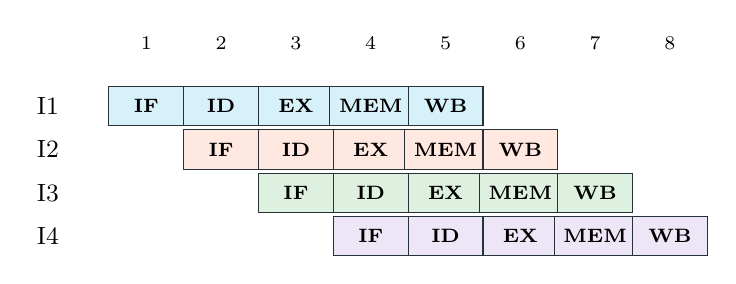
\begin{tikzpicture}[s/.style={draw=brandDark, minimum width=0.95cm, minimum height=0.5cm, font=\codefont\scriptsize\bfseries}]
        \foreach \c in {1,...,8} \node[font=\codefont\scriptsize] at (0.95*\c, 0.35) {\c};
        \foreach \i/\col in {1/brandTeal, 2/brandOrange, 3/brandGreen, 4/brandPurple} {
            \node[font=\small] at (-0.3,-0.55*\i+0.1) {I\i};
            \foreach \st [count=\k from 0] in {IF, ID, EX, MEM, WB} {
                \pgfmathsetmacro\x{0.95*(\i+\k)}
                \node[s, fill=\col!25] at (\x, -0.55*\i+0.1) {\st};
            }
        }
    \end{tikzpicture}
    \end{center}
    \begin{tbox}{\faLightbulb\quad Cycles}
        without: $n \times k$ \qquad with: $k + (n - 1)$. \quad 100 instructions, 5 stages: 500 vs 104 (4.8 times faster).
    \end{tbox}
\end{frame}

\begin{frame}{Hazards}
    \begin{itemize}
        \item \textbf{Data}: \code{add rax, rbx} then \code{add rcx, rax}: forward the result, or wait.
        \item \textbf{Control}: after a jump, fetched instructions may be wrong: \textbf{branch prediction}.
        \item \textbf{Structural}: two instructions need the same circuit at once.
    \end{itemize}
\end{frame}

\begin{frame}{\code{mov}, \code{add}, \code{jmp} in the pipeline}
    \begin{center}
    \small
    \begin{tabularx}{\linewidth}{|c|L|L|L|}
        \hline \ras{} & \ras{\code{mov rax, 60}} & \ras{\code{add rax, rbx}} & \ras{\code{jmp fin}} \\ \hline
        IF & 48 C7 C0 3C 00 00 00 & 48 01 D8 & EB 00 \\ \hline
        ID & 64 bits, value in the instruction & read RAX and RBX & short jump \\ \hline
        EX & -- & RAX + RBX, flags & target = RIP + 0 \\ \hline
        WB & \nql{RAX}{60} & RAX gets the result & RIP gets the target \\ \hline
    \end{tabularx}
    \end{center}
    A Core i7 has 14+ stages, starts 4 instructions per cycle, and runs them out of order.
\end{frame}

\begin{frame}{Practice}
    \begin{obox}{\faEdit\quad Try it}
        \begin{enumerate}
            \item RAX = \hex{FFFF\dots FFFF}, then \code{mov eax, 1}: RAX? \hfill \textcolor{brandMuted}{\hex{0000000000000001}}
            \item Address of element 10 of an \code{int} array at \hex{601000}? \hfill \textcolor{brandMuted}{\hex{601028}}
            \item 1000 instructions, 6 stages: cycles with a pipeline? \hfill \textcolor{brandMuted}{1005}
        \end{enumerate}
    \end{obox}
\end{frame}

\begin{frame}{Summary}
    \begin{tbox}{\faCheckCircle\quad Remember}
        \begin{itemize}
            \item x86-64: 16 registers of 64 bits, flat memory.
            \item address $=$ base $+$ index $\times$ scale $+$ displacement.
            \item SIMD: several numbers at once; pipeline: overlapping steps.
        \end{itemize}
    \end{tbox}
\end{frame}

\end{document}
